\section{Radiodifusión en AM}
\label{sec:am}

\subsection{Modulación AM}
En la modulación de amplitud con doble banda lateral y portadora completa, la envolvente de la portadora sigue a la señal modulante. Para un tono de frecuencia $f_m$ y un índice de modulación $m$, se cumple:
\begin{equation}
    v_{AM} = E_c \left[1 + m \cos(2\pi f_m t)\right] \cos(2\pi f_c t)
    = E_c \cos(2\pi f_c t) + \frac{m E_c}{2} \cos\left[2\pi (f_c \pm f_m) t\right]
    \label{eq:am}
\end{equation}

El espectro tiene tres componentes (\autoref{fig:am_teoria}, izquierda): 
\begin{itemize}
    \item \underline{La portadora}, en $f_c$, con amplitud $E_c$. No depende de la modulación y concentra al menos dos tercios de la potencia, aun con $m = 1$.
    \item \underline{Las bandas laterales inferior y superior}, en $f_c - f_m$ y $f_c + f_m$, con amplitud $m E_c / 2$ cada una. Llevan la información y son imágenes especulares una de la otra, es decir, hay una simetría exacta entre las dos bandas laterales.
\end{itemize}
En dBc (decibelios relativos a la portadora), cada banda lateral queda $20 \log(2/m)$ por debajo de la portadora: $6 \, [dB]$ con $m = 1$ y $12 \, [dB]$ con $m = 0{,}5$. Con una señal AM el resultado es un espectro continuo y simétrico alrededor de la portadora, que ocupa $2 f_{m,max}$ (\autoref{fig:am_teoria}, derecha).

\begin{figure}[H]
    \centering
    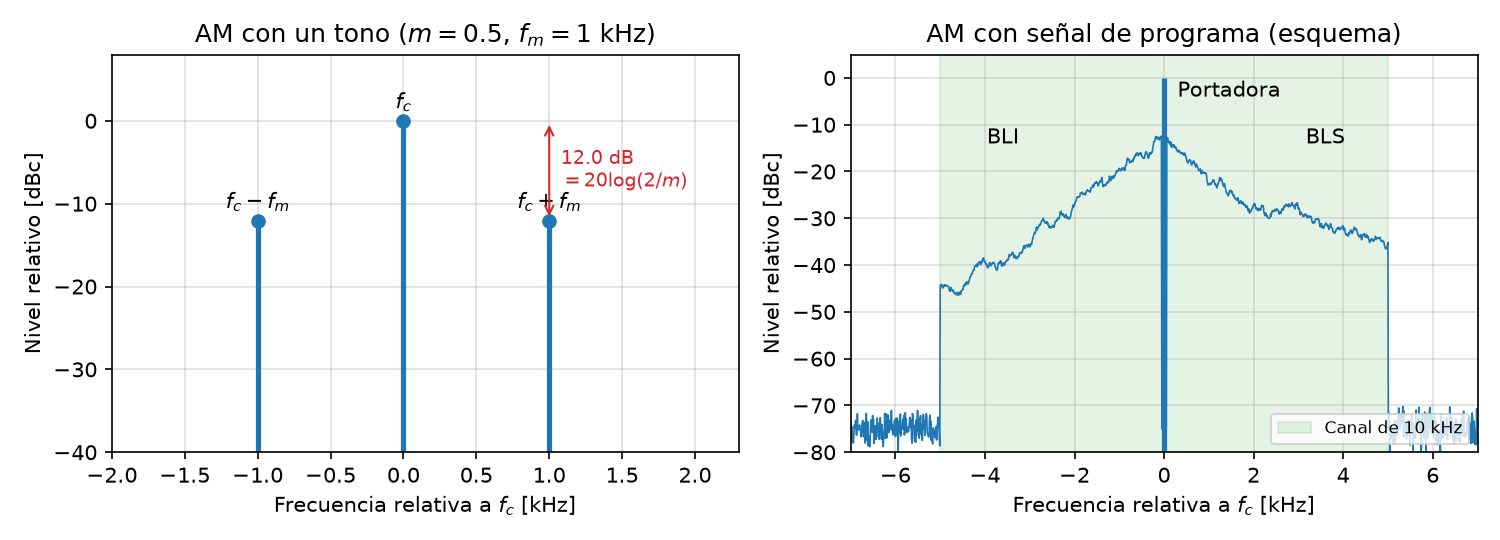
\includegraphics[width=\textwidth]{teoria/am_espectro.png}
    \caption{Espectro de AM con un tono (esquemas propios).}
    \label{fig:am_teoria}
\end{figure}

\subsection{Mediciones}

\subsubsection*{Exploración de la banda e identificación de las emisoras}
Se exploró la banda de radiodifusión en AM, que se extiende de $535$ a $1705 \, [kHz]$.

\begin{table}[H]
    \centering
    \caption{Configuración del analizador y resultados en la banda de AM.}
    \label{tab:am_resultados}
    \begin{tabular}{p{8.5cm} p{5.8cm}}
        \toprule
        \textbf{Parámetro} & \textbf{Valor} \\
        \midrule
        Frecuencias de inicio y fin & $557{,}5$ a $1727{,}5 \, [kHz]$ \\
        Frecuencia central & $1142{,}5 \, [kHz]$ \\
        \textit{Span} & $1{,}17 \, [MHz]$ \\
        Nivel de referencia & $-90 \, [dBm]$ \\
        RBW / VBW & $300 \, [Hz]$ / $30 \, [kHz]$ \\
        \midrule
        \textbf{Emisora 1} \\
        \midrule
        Frecuencia de la portadora & $700 \, [kHz]$ \\
        Emisora identificada & Cadena 3 - Córdoba \\
        \textit{Span} & $20 \, [kHz]$ \\
        Nivel de referencia & $-98 \, [dBm]$ \\
        RBW / VBW & $300 \, [Hz]$ / $10 \, [kHz]$ \\
        Nivel de la portadora & $-101 \, [dBm]$ \\
        \midrule
        \textbf{Emisora 2} \\
        \midrule
        Frecuencia de la portadora & $810 \, [kHz]$ \\
        Emisora identificada & Radio Mitre - Córdoba \\
        \textit{Span} & $20 \, [kHz]$ \\
        Nivel de referencia & $-98 \, [dBm]$ \\
        RBW / VBW & $300 \, [Hz]$ / $10 \, [kHz]$ \\
        Nivel de la portadora & $-102 \, [dBm]$ \\
        \bottomrule
    \end{tabular}
\end{table}

\begin{figure}[H]
    \centering
    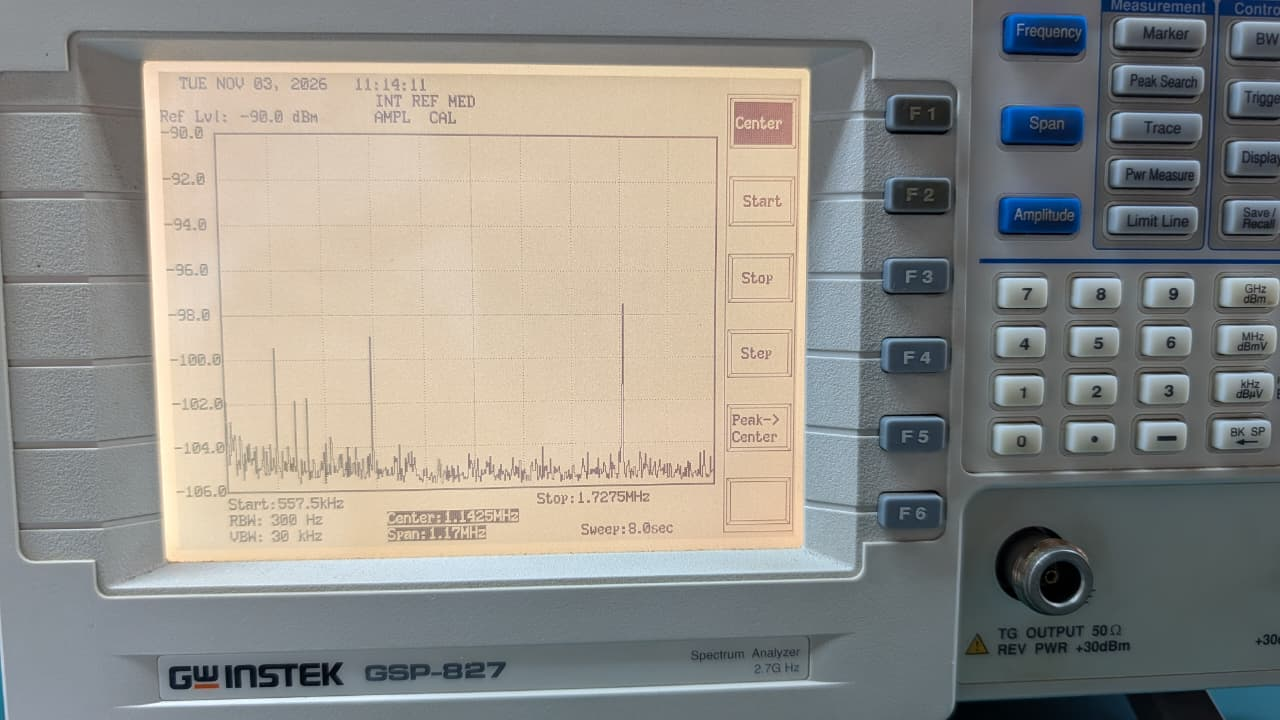
\includegraphics[width=0.85\textwidth]{am_completa.png}
    \caption{Exploración de la banda de radiodifusión en AM.}
    \label{fig:am_completa}
\end{figure}

\begin{figure}[H]
    \centering
    \begin{subfigure}[b]{0.49\textwidth}
        \centering
        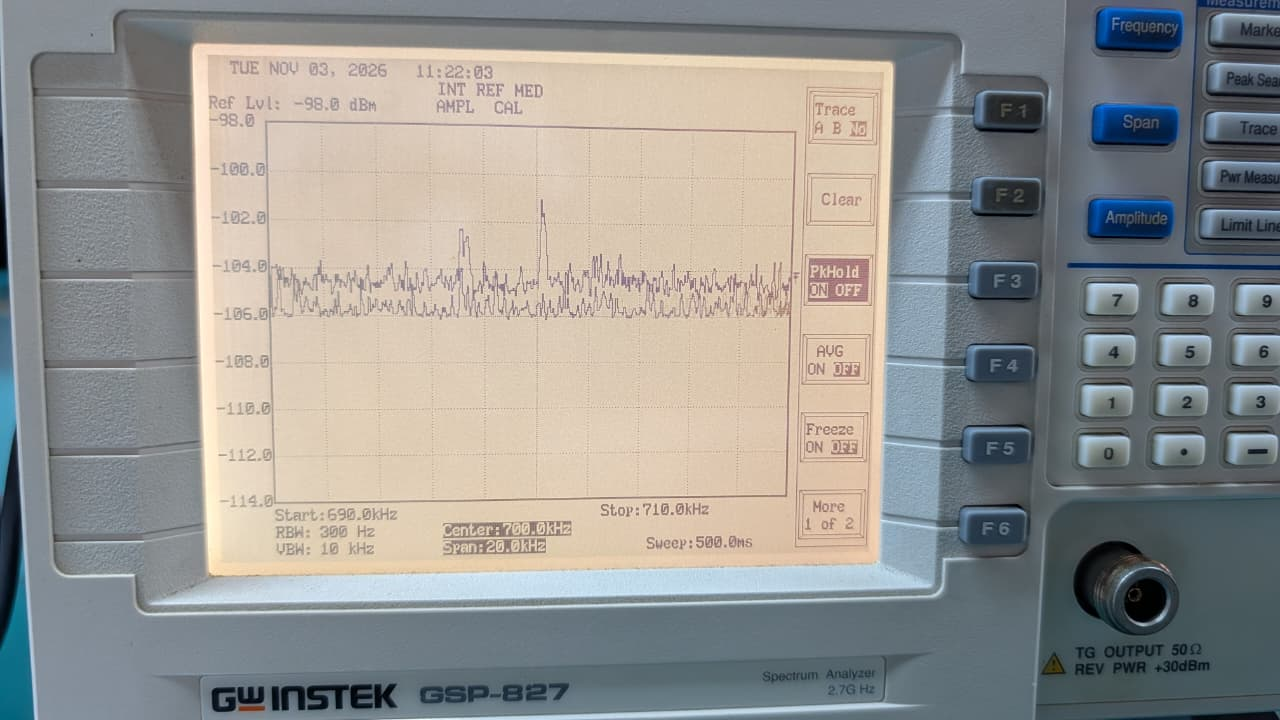
\includegraphics[width=\linewidth]{am_emisora1.png}
        \caption{Emisora 1 (Cadena 3, $700 \, [kHz]$).}
        \label{fig:am_emisora1}
    \end{subfigure}
    \hfill
    \begin{subfigure}[b]{0.49\textwidth}
        \centering
        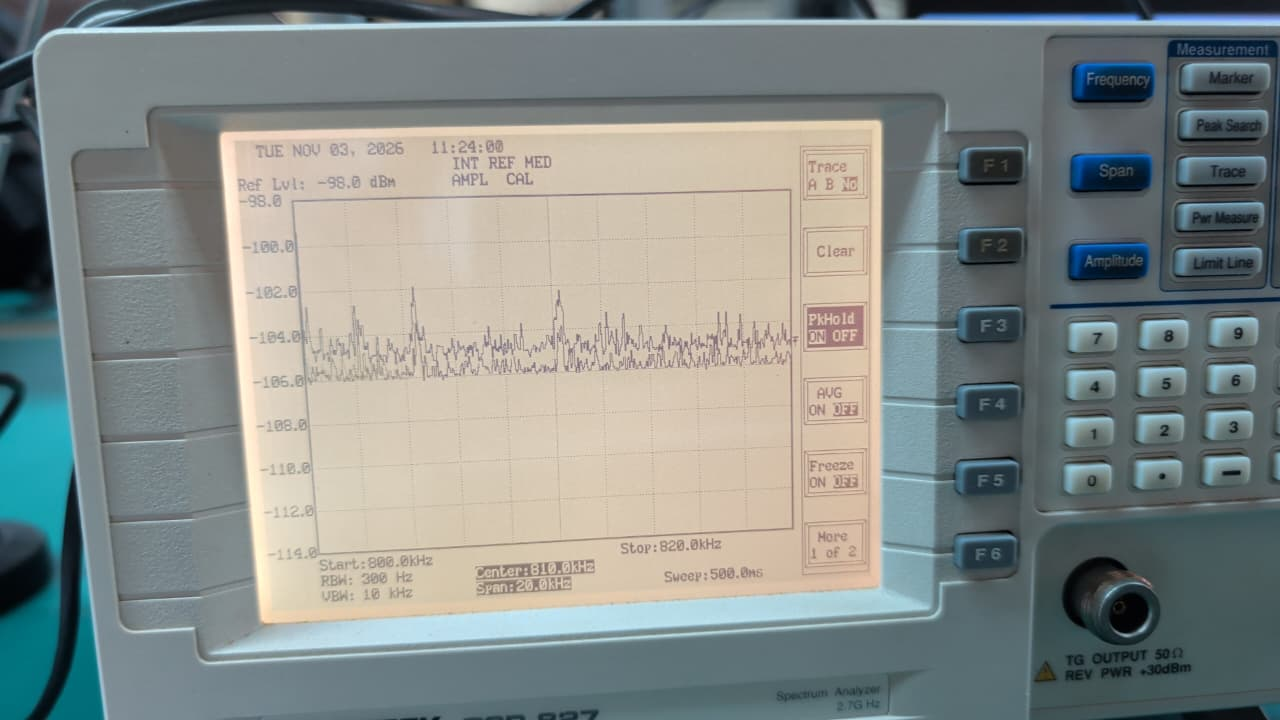
\includegraphics[width=\linewidth]{am_emisora2.png}
        \caption{Emisora 2 (Radio Mitre, $810 \, [kHz]$).}
        \label{fig:am_emisora2}
    \end{subfigure}
    \caption{Portadoras de las emisoras de AM observadas con un \textit{span} de $20 \, [kHz]$.}
    \label{fig:am_emisoras}
\end{figure}

\subsubsection*{Señal AM generada en el laboratorio}
Para observar el espectro de una AM con una modulante conocida, se conectó al analizador un generador de funciones GW Instek AFG-2125 con modulación interna (\autoref{fig:am_gen_parametros}).

\begin{table}[H]
    \centering
    \caption{Configuración del generador y del analizador para la señal AM generada.}
    \label{tab:am_generador}
    \begin{tabular}{p{8.5cm} p{5.8cm}}
        \toprule
        \textbf{Parámetro} & \textbf{Valor} \\
        \midrule
        \textbf{Generador (AFG-2125)} \\
        \midrule
        Portadora & $580 \, [kHz]$, $-20 \, [dBm]$ \\
        Modulante & $10 \, [kHz]$, senoidal y cuadrada (interna) \\
        Profundidad de modulación & $80 \, $\% ($m = 0{,}8$) \\
        \midrule
        \textbf{Analizador (GSP-827)} \\
        \midrule
        Frecuencia central / \textit{span} & $582 \, [kHz]$ / $1 \, [MHz]$ \\
        Nivel de referencia & $-20 \, [dBm]$ \\
        RBW / VBW & $9 \, [kHz]$ / $100 \, [kHz]$ \\
        Nivel de la portadora & $\approx -31 \, [dBm]$ \\
        Marcador en $674{,}5 \, [kHz]$ (senoidal / cuadrada) & $-73{,}7 \, [dBm]$ / $-56{,}1 \, [dBm]$ \\
        \bottomrule
    \end{tabular}
\end{table}

\begin{figure}[H]
    \centering
    \begin{subfigure}[b]{0.49\textwidth}
        \centering
        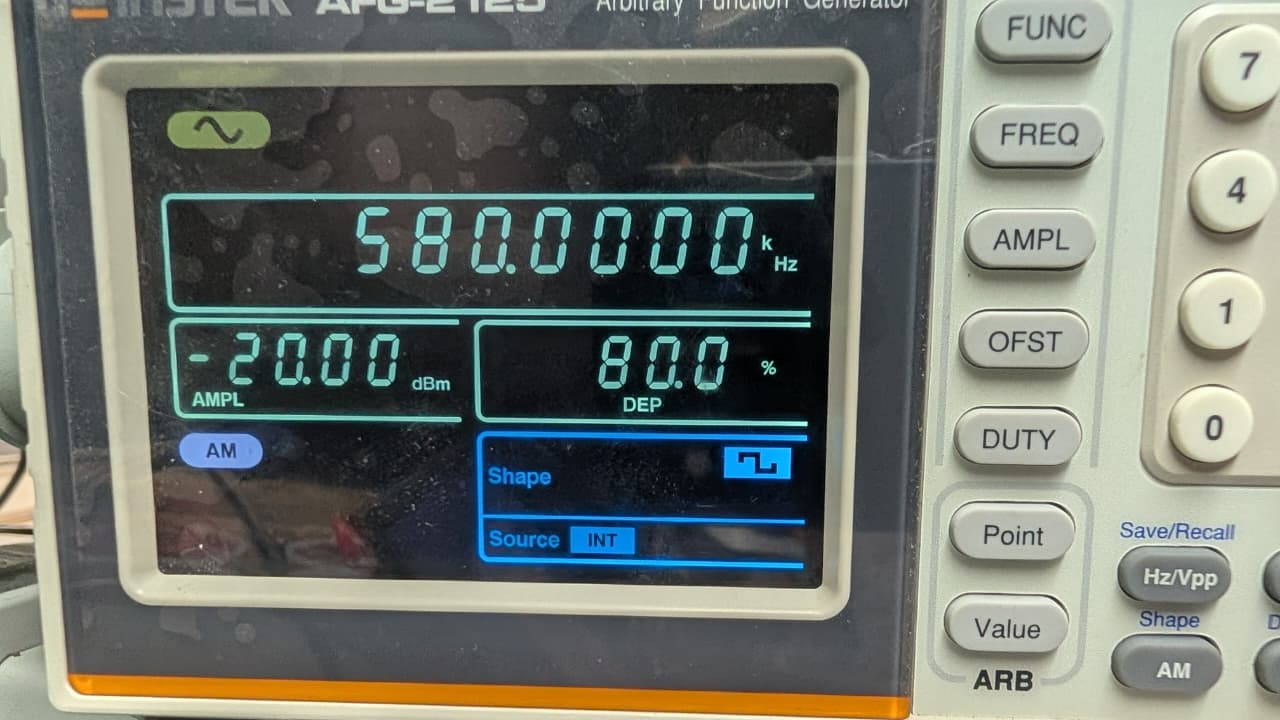
\includegraphics[width=\linewidth]{am_gen_portadora.png}
        \caption{Portadora.}
    \end{subfigure}
    \hfill
    \begin{subfigure}[b]{0.49\textwidth}
        \centering
        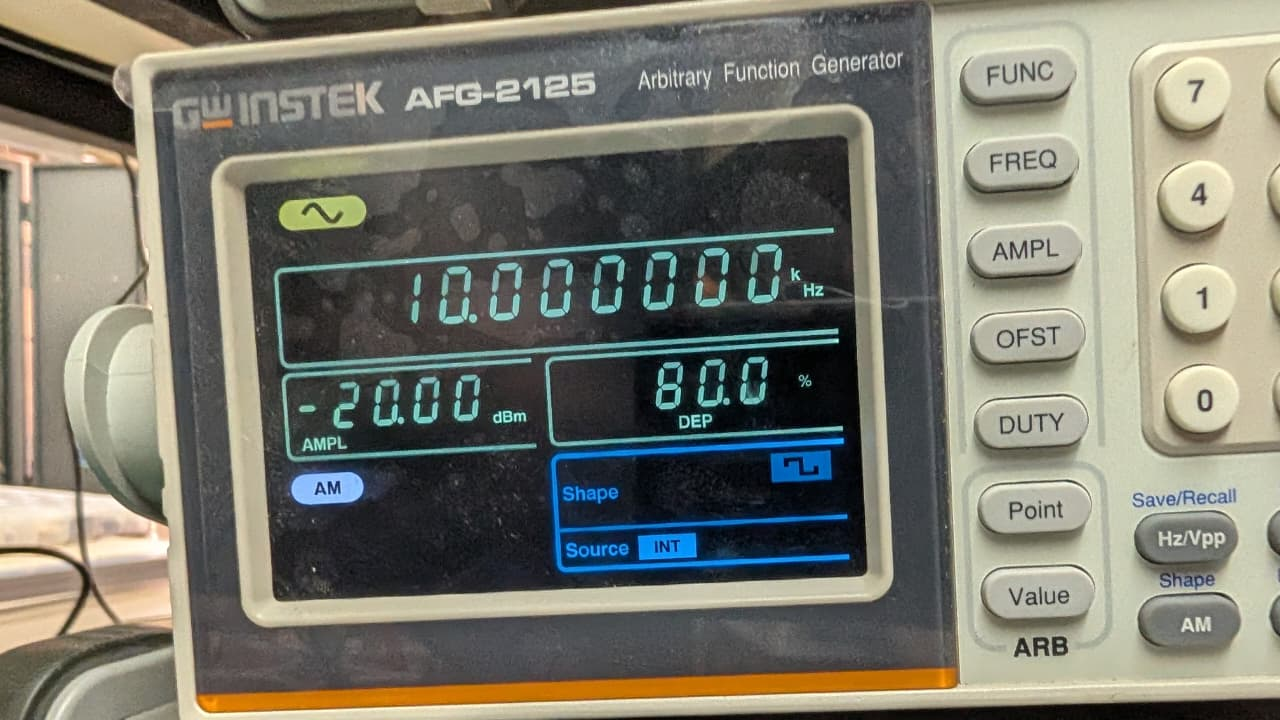
\includegraphics[width=\linewidth]{am_gen_modulante.png}
        \caption{Modulante.}
    \end{subfigure}
    \caption{Configuración del generador AFG-2125.}
    \label{fig:am_gen_parametros}
\end{figure}

\begin{figure}[H]
    \centering
    \begin{subfigure}[b]{0.49\textwidth}
        \centering
        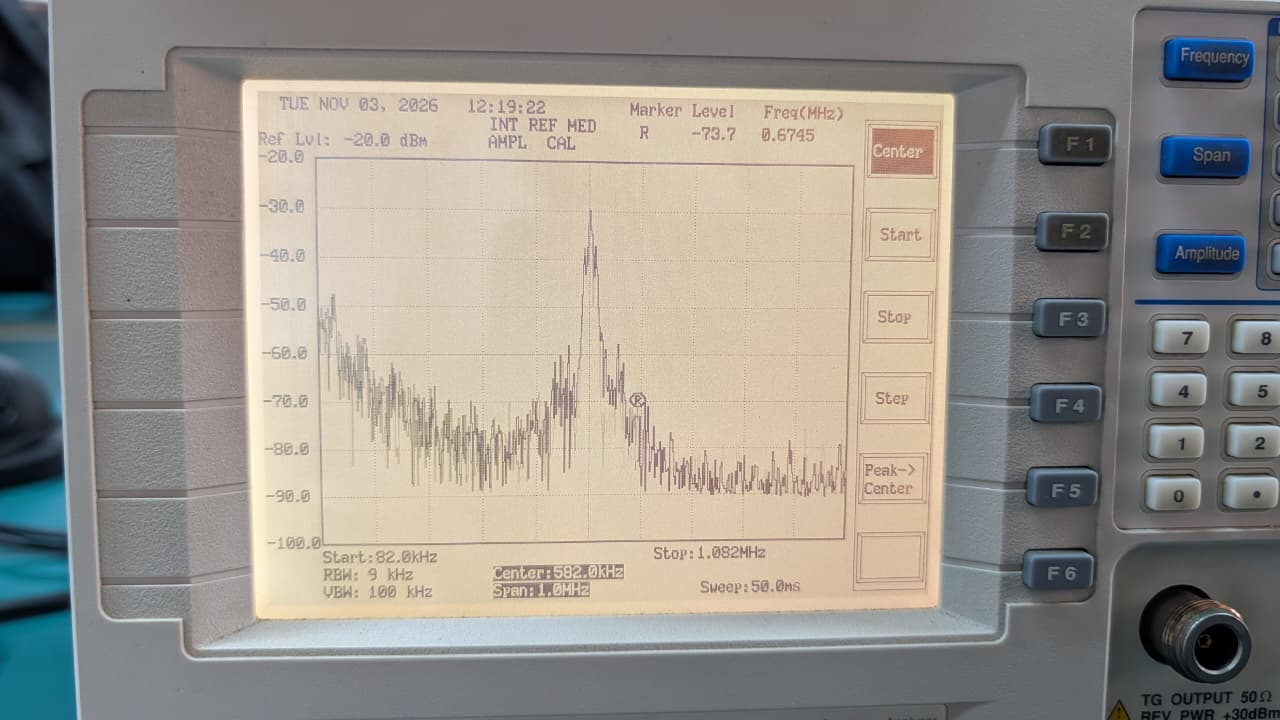
\includegraphics[width=\linewidth]{am_gen_seno.png}
        \caption{Modulante senoidal.}
        \label{fig:am_gen_seno}
    \end{subfigure}
    \hfill
    \begin{subfigure}[b]{0.49\textwidth}
        \centering
        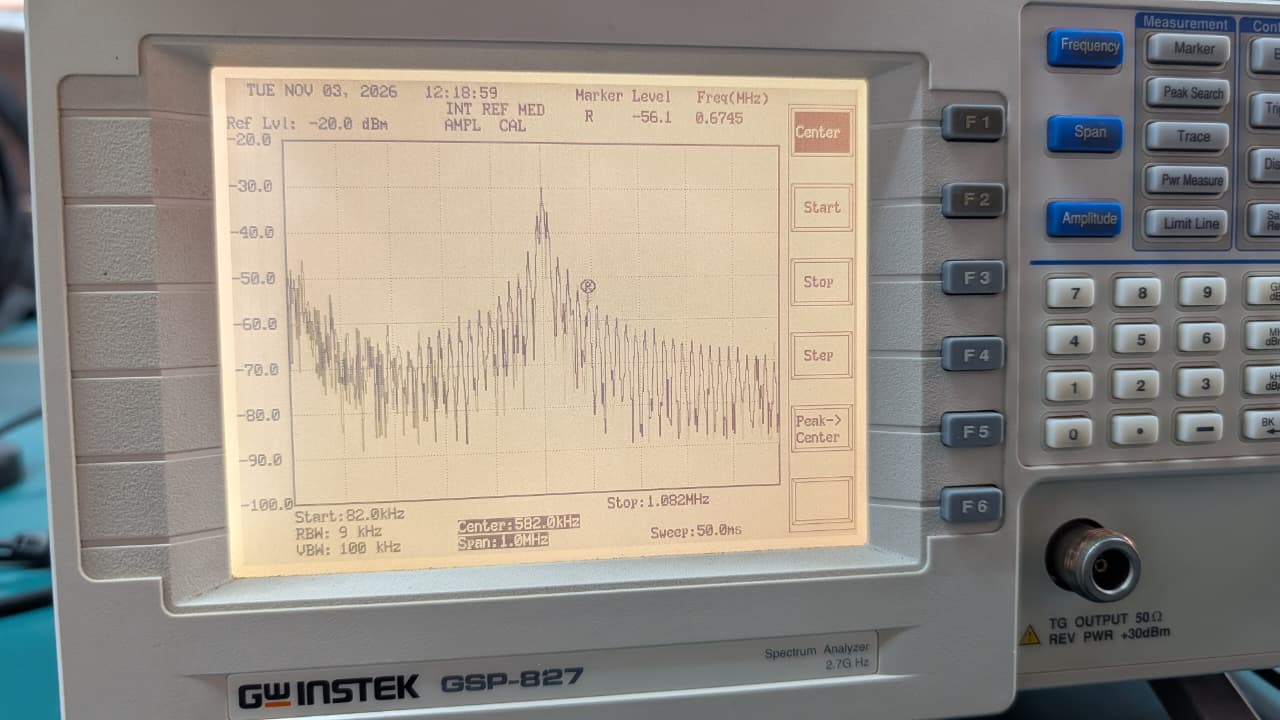
\includegraphics[width=\linewidth]{am_gen_cuadrada.png}
        \caption{Modulante cuadrada.}
        \label{fig:am_gen_cuadrada}
    \end{subfigure}
    \caption{Espectro de la señal AM generada ($f_c = 580 \, [kHz]$, $f_m = 10 \, [kHz]$, $m = 0{,}8$).}
    \label{fig:am_gen}
\end{figure}


\subsection{Análisis}

\subsubsection*{Componentes del espectro}
En las \autoref{fig:am_emisora1} y~\ref{fig:am_emisora2} se distingue la portadora en la frecuencia asignada a cada emisora, pero no las bandas laterales. La portadora se recibió con unos $-101$ a $-102 \, [dBm]$ pero las bandas laterales quedaron por debajo del piso de ruido y no pudieron observarse.

Se utilizó la retención de máximos (\textit{Peak Hold}), que conserva para cada frecuencia el mayor valor registrado en los barridos sucesivos. Esto permite acumular la envolvente de una emisión variable, pero también retiene los picos del ruido.

El bajo nivel recibido se atribuye a la antena utilizada (\autoref{fig:am_antena}): una antena interior de dos varillas en V, que es un dipolo pensado para los canales de VHF, donde cada varilla mide de un cuarto de longitud de onda. En la banda de AM, en cambio, $\lambda \approx 430 \, [m]$ en $700 \, [kHz]$, y con las varillas extendidas hasta un largo total de $1 \, [m]$ resulta $L / \lambda \approx 0{,}002$. A esto se suma la atenuación de la recepción en el interior del edificio.

\begin{figure}[H]
    \centering
    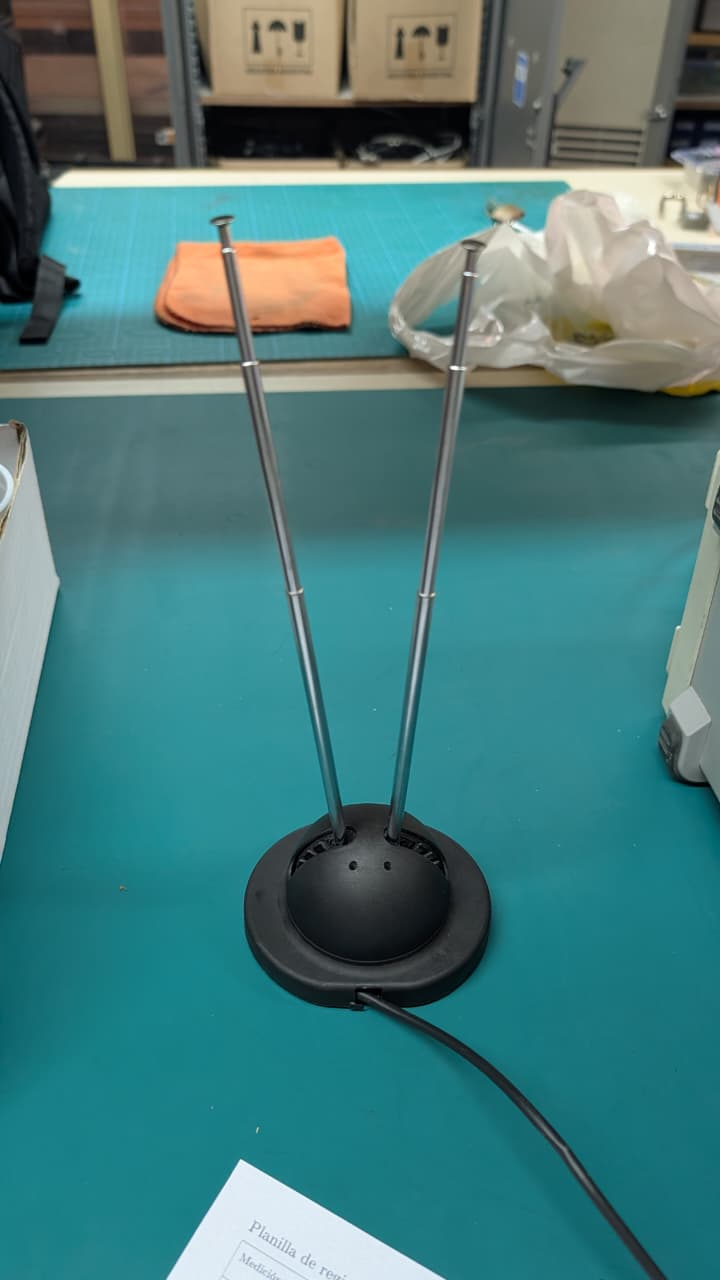
\includegraphics[width=0.25\textwidth]{am_antena.png}
    \caption{Antena interior de varillas telescópicas utilizada para la recepción en AM.}
    \label{fig:am_antena}
\end{figure}

\subsubsection*{Ancho de banda ocupado}
Para el ancho de banda se había previsto el criterio de ``$x$ dB'' de la Recomendación UIT-R SM.328, que lo mide entre las frecuencias donde el espectro cae $26 \, [dB]$ por debajo del máximo \cite{itu_sm328, itu_sm443}. Aplicarlo requiere que la portadora supere el piso de ruido en al menos $26 \, [dB]$, y en esta medición la diferencia fue de unos $3 \, [dB]$. Por eso el ancho de banda ocupado no pudo medirse. Según la canalización del CABFRA, con una separación de $10 \, [kHz]$ entre canales, se espera que la emisión ocupe como máximo unos $10 \, [kHz]$ \cite{cabfra}.

\subsubsection*{Canales adyacentes}
En las capturas con \textit{span} de $20 \, [kHz]$, los bordes de la pantalla coinciden con los canales adyacentes a $\pm 10 \, [kHz]$ de cada portadora, y en ninguno de ellos se observó una portadora. En el barrido de toda la banda (\autoref{fig:am_completa}) tampoco aparecen portadoras a $\pm 20 \, [kHz]$: las demás emisoras visibles están separadas varias decenas de kHz. Esto es coherente con la planificación, que evita asignar canales adyacentes a emisoras de una misma zona para limitar la interferencia entre ellas.

Se tuvo como limitación al piso de ruido: una emisora adyacente que llegue con menos de unos $-104 \, [dBm]$ no puede distinguirse, de modo que la ausencia de portadoras sólo indica que no hay señales por encima de ese nivel con la antena utilizada.

\subsubsection*{Máxima frecuencia modulante}
Con la separación de $10 \, [kHz]$ entre canales del CABFRA \cite{cabfra}, una emisión de doble banda lateral que no invada los canales adyacentes debe limitarse a unos $5 \, [kHz]$. Para verificarlo experimentalmente, la portadora debería superar el piso de ruido en varias decenas de dB, y el ancho debería medirse en retención de máximos durante el tiempo suficiente para que aparezcan las frecuencias altas del programa.

\subsubsection*{Señal AM generada: modulante senoidal y cuadrada}
Con una modulante senoidal, la \autoref{eq:am} predice una portadora y dos bandas laterales en $f_c \pm f_m = 570$ y $590 \, [kHz]$, con un nivel de $20 \log \frac{0{,}8}{2} \approx -8 \, [dBc]$ y un ancho de banda de $2 f_m = 20 \, [kHz]$. 

En la \autoref{fig:am_gen_seno}, sin embargo, se observa un único pico: las bandas laterales están a $10 \, [kHz]$ de la portadora, separación comparable al RBW de $9 \, [kHz]$, y con un \textit{span} de $1 \, [MHz]$. 

Se asume que hubo una configuración incorrecta del analizador, ya que no pudieron observarse las bandas laterales, por lo que el índice de modulación no pudo verificarse.

Con una modulante cuadrada, la envolvente alterna entre $1 + m$ y $1 - m$. Su serie de Fourier contiene sólo armónicas impares, de amplitud $\frac{4}{n \pi}$, de modo que cada una produce un par de bandas laterales en $f_c \pm n f_m$ con un nivel de
\begin{equation}
    N_{BL,n} - N_c = 20 \log \left( \frac{m}{2} \cdot \frac{4}{n \pi} \right), \qquad n = 1, 3, 5, \dots
    \label{eq:am_cuadrada}
\end{equation}

\begin{table}[H]
    \centering
    \caption{Nivel teórico de las bandas laterales con modulante cuadrada ($m = 0{,}8$, $f_m = 10 \, [kHz]$).}
    \label{tab:am_cuadrada}
    \begin{tabular}{c c c}
        \toprule
        \textbf{Armónica $n$} & \textbf{Frecuencias $[kHz]$} & \textbf{Nivel $[dBc]$} \\
        \midrule
        1 & $570$ y $590$ & $-5{,}9$ \\
        3 & $550$ y $610$ & $-15{,}4$ \\
        5 & $530$ y $630$ & $-19{,}8$ \\
        7 & $510$ y $650$ & $-22{,}8$ \\
        9 & $490$ y $670$ & $-24{,}9$ \\
        \bottomrule
    \end{tabular}
\end{table}

El espectro de la \autoref{fig:am_gen_cuadrada} coincide con esta predicción: un peine de componentes separadas $2 f_m = 20 \, [kHz]$, cuyo nivel disminuye lentamente y que se extiende por todo el \textit{span}.

La comparación muestra el efecto del contenido armónico de la modulante sobre el ancho de banda. Una senoidal ocupa $2 f_m$, mientras que una cuadrada, por sus flancos abruptos, tiene en teoría un ancho de banda infinito: en la práctica, uno que se extiende hasta donde sus armónicas caen bajo el piso de ruido. Por eso en radiodifusión el audio se limita en banda antes de modular, de modo que la emisión no invada los canales adyacentes.

\subsubsection*{Índice de modulación en una emisión de programa}
Con un único tono sinusoidal, el índice de modulación se obtiene de la diferencia de nivel entre una banda lateral y la portadora, a partir de la \autoref{eq:am}:
\begin{equation}
    m = \frac{2 E_{BL}}{E_c} = 2 \cdot 10^{(N_{BL} - N_c)/20}
    \label{eq:indice_am}
\end{equation}
Con una emisión comercial la \autoref{eq:indice_am} no puede aplicarse, porque la modulante no es un tono: tiene muchas componentes de frecuencia y amplitud variables, que reparten la potencia de las bandas laterales en un espectro continuo. No hay una única línea de banda lateral para medir, y su nivel depende del RBW y del instante. Tampoco puede suponerse que una emisora comercial module con $m = 1$: los procesadores de audio limitan los picos por debajo de la sobremodulación, y el índice varía todo el tiempo con el programa.

\subsection{Síntesis}
La AM imprime la información en la amplitud de la portadora. En el espectro esto se traduce en una portadora fija y dos bandas laterales simétricas, cuyo ancho es el doble de la máxima frecuencia modulante y cuyo nivel depende del índice de modulación.

En las emisoras recibidas, con una antena poco adecuada para la banda, sólo la portadora superó el piso de ruido, mientras que las bandas laterales, de menor nivel y repartidas en varios kHz, quedaron ocultas. Las emisoras se identificaron por su frecuencia, pero el ancho de banda y la máxima frecuencia modulante quedaron limitados al análisis teórico.

Con la señal del generador, en cambio, la modulante cuadrada produjo el peine de bandas laterales en las armónicas impares que predice su serie de Fourier, lo que muestra que el ancho de banda de una AM depende del contenido espectral de la modulante y justifica la limitación del audio en radiodifusión. Con la modulante senoidal, la configuración del analizador no permitió resolver las bandas laterales, por lo que el índice de modulación no pudo verificarse experimentalmente.